% !TeX spellcheck = en_US
%\documentclass[11pt,a4paper]{article}
\documentclass[11pt
  , a4paper
  , article
  , oneside
%  , twoside
%  , draft
]{memoir}

\usepackage{control}
\usepackage{kotex}
\usepackage[numbers]{natbib}
%\usepackage[pdftex]{graphicx}
%\DeclareGraphicsExtensions{.pdf,.png,.jpg}
\begin{document}

\newcommand{\technumber}{
  Low-Power Real-Time Scheduling\\
  Document 1: 2016-06-02}
\title{\textbf{Real-Time Dynamic Voltage Scaling for Low-Power \\
		Embedded Operating Systems \\
		요약 \\}}

\author{이상일\thanks{silee7103@ibs.re.kr} \\

  학번: 201460437\\
  Computer Engineering, Chungnam National University 
}
\date{\today}

\renewcommand{\maketitlehooka}{\begin{flushright}\textsf{\technumber}\end{flushright}}
%\renewcommand{\maketitlehookb}{\centering\textsf{\subtitle}}
%\renewcommand{\maketitlehookc}{C}
%\renewcommand{\maketitlehookd}{D}

\maketitle

\begin{abstract}
MATLAB을 사용한 Digital Signal Processing에 대한 실습과제에 대한 Documents를 구성한다.
\end{abstract}

\chapter{Example 4-10:}

\begin{lstlisting}[style=termstyle]
%Example 4-10
b = [1, 0.4*sqrt(2)]; a = [1,-0.8*sqrt(2),0.64];
[R,p,C] = residuez(b,a)

Mp = (abs(p))'
Ap = (angle(p))'/pi
[delta, n]=impseq(0,0,6);
x = filter(b,a,delta)
x = ((0.8).^n).*(cos(pi*n/4)+2*sin(pi*n/4))\end{lstlisting}

\begin{figure}[h!]
	\centering
	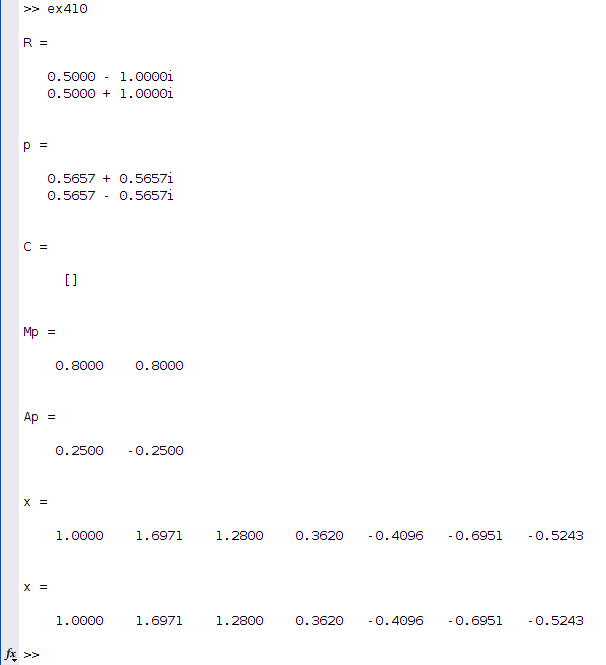
\includegraphics[width=0.4\textwidth,height=0.15\textwidth]{./images/ex410.png}
	\caption{Example 4.10 Result}
	\label{fig:Example 4.10 Result}
\end{figure}

위 계산으로 부터,
 
\begin {equation}
X(z) =\frac{0.5-j}{1-0.8e^{j\frac{\pi}{4}z^{-1}}}+\frac{0.5+j}{1-0.8e^{-j\frac{\pi}{4}z^{-1}}}, |z| > 0.8
\end {equation}

그리고, 역변환을 다음과 같이 얻는다.
\begin {equation}
x(n) = 0.8^n[cos(\frac{\pi*n}{4})+2sin(\frac{\pi*n}{4})]u(n)
\end {equation}


\chapter{Example 4-11a:}
\subsection{4-11a}
\begin{lstlisting}[style=termstyle]
Example 4.11a
b = [1,0]; a = [1, -0.9];
zplane(b,a)\end{lstlisting}

\begin{figure}[h!]
	\centering
	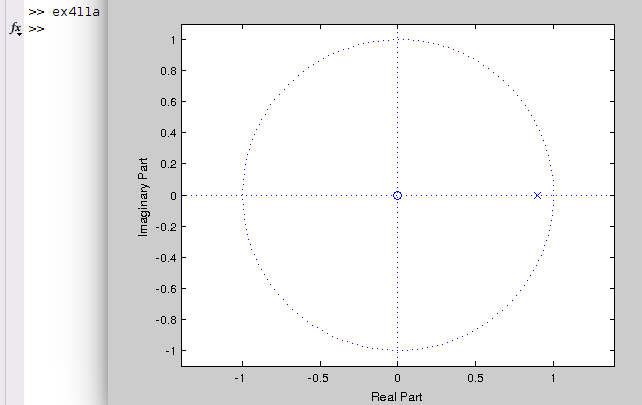
\includegraphics[width=0.5\textwidth,height=0.3\textwidth]{./images/ex411-a.png}
	\caption{Example 4.11a Result}
	\label{fig:Example 4.11a Result}
\end{figure}

\subsection{4-11b}
\begin{lstlisting}[style=termstyle]
%Example 4.11-b

b = [1,0]; a = [1, -0.9];
[H, w]= freqz(b,a, 100);
magH=abs(H); phaH = angle(H);

%[H,w]=freqz(b,a,200,'whole');
%magH=abs(H(1:101)); phaH=angle(H(1:101));

%w = [0:1:100]*pi/100; H = freqz(b,a,w);

subplot(2,1,1); plot(w/pi,magH); grid;
xlabel('frequency in pi units'); ylabel('Magnitude');
title('Magnitude Response');

subplot(2,1,2); plot(w/pi,phaH/pi); grid;
xlabel('frequency in pi units'); ylabel('Phase in pi units');
title('Phase Response');
\end{lstlisting}

\begin{figure}[h!]
	\centering
	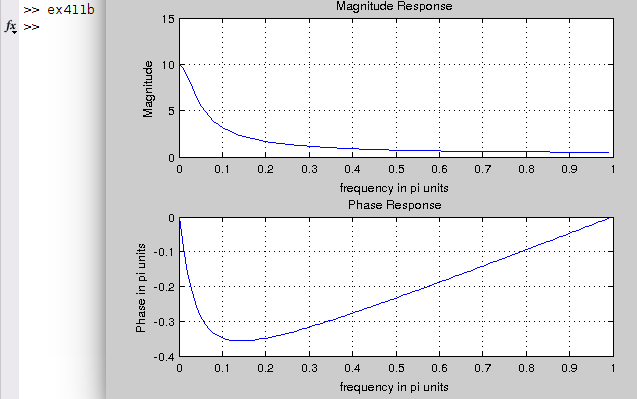
\includegraphics[width=0.5\textwidth,height=0.3\textwidth]{./images/ex411b.png}
	\caption{Example 4.11b Result}
	\label{fig:Example 4.11b Result}
\end{figure}

\subsection{4-11b2}
\begin{lstlisting}[style=termstyle]
%Example 4.11-b

b = [1,0]; a = [1, -0.9];
w = [0:1:100]*pi/100; H = freqz(b,a,w);

subplot(2,1,1); plot(w/pi,magH); grid;
xlabel('frequency in pi units'); ylabel('Magnitude');
title('Magnitude Response');

subplot(2,1,2); plot(w/pi,phaH/pi); grid;
xlabel('frequency in pi units'); ylabel('Phase in pi units');
title('Phase Response');
\end{lstlisting}

\begin{figure}[h!]
	\centering
	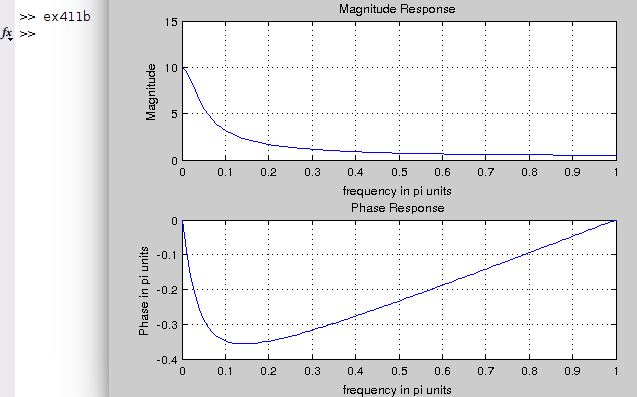
\includegraphics[width=0.5\textwidth,height=0.3\textwidth]{./images/ex411-b2.png}
	\caption{Example 4.11b2 Result}
	\label{fig:Example 4.11b2 Result}
	\end{figure}

\subsection{4-11c}
z-변환표로 부터,
\begin {equation}
ㅗ(n) = Z^{-1}[\frac{1}{1-0.9z^{-1}}, |z|> 0.9] = (0.9)^nu(n)
\end {equation}

\clearpage

\chapter{Example 4-12:}
\subsection{4-12a: 전달함수 표현}

\begin {equation}
H(e^{jw}) = \frac{e^{jw}+1}{e^{jw}-0.9e^{jw} +0.81} = \frac{e^{jw}+1}{(e^{jw}-0.9e^{j\pi/3})(e^{jw}-0.9e^{-j\pi/3})}
\end {equation}

\subsection{4-12b: 차분방정식 표현}
\begin {equation}
\frac{Y(z)}{X(z)} = \frac{z^{-1} + z^{-2}}{1-0.9z^{-1}+0.81z^{-2}}
\end {equation}

\subsection{4-12c: 임펄스 응답 표현}

\begin{lstlisting}[style=termstyle]
%Example 4.12

b = [0,1,1]; a = [1, -0.9, 0.81];
[R,p,C]=residuez(b,a)

Mp = (abs(p))'
Ap = (angle(p))'/pi
\end{lstlisting}

\begin{figure}[h!]
	\centering
	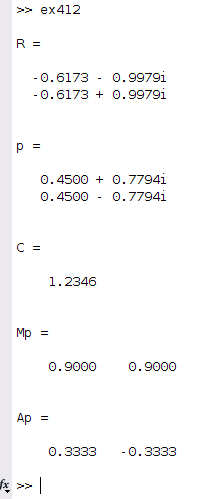
\includegraphics[width=0.3\textwidth,height=0.15\textwidth]{./images/ex412.png}
	\caption{Example 4.12 Result}
	\label{fig:Example 4.12 Result}
\end{figure}

\chapter{Example 4-13:}
\subsection{4-13a: 시스템 함수}

\begin {equation}
H(z) = \frac{1-z^{-2}}{(1+0.9z^{-1})(1-0.9z^{-1})}
\end {equation}

\subsection{4-13b: 단위 임펄스 응답}
\begin{lstlisting}[style=termstyle]
%Example 4.13

b = [1,0,-1]; a = [1, 0, -0.81];
[R,p,C]=residuez(b,a)

\end{lstlisting}


\subsection{4-13c: 단위계단 응답}
Z 변환표로 부터,

\begin {equation}
V(z) = \frac{1+z^{-1}}{(1+0.9z^{-1})(1-0.9z^{-1})}, |z| > 0.9
\end {equation}
또는,
\begin {equation}
V(z) = 1.0556\frac{1}{(1-0.9z^{-1})} - 0.0556\frac{1}{1+0.9z^{-1}}, |z| > 0.9
\end {equation}

\begin {equation}
v(n) = [1.0556(0.9)^n - 0.0556(-0.9)^n]u(n)
\end {equation}

\subsection{4-13d: 주파수 응답}
\begin{lstlisting}[style=termstyle]
%Example 4.13

b = [1,0,-1]; a = [1, 0, -0.81];
[R,p,C]=residuez(b,a)

w = [0:1:500]*pi/500; H = freqz(b,a,w);
magH = abs(H); phaH = angle(H);

subplot(2,1,1); plot(w/pi,magH); grid
xlabel('Freq. in pi units'); ylabel('Magnitude');
title('Magnitude Response');

subplot(2,1,2); plot(w/pi,phaH/pi); grid
xlabel('Freq. in pi units'); ylabel('Phase in pi units');
title('Phase Response');
\end{lstlisting}
\begin{figure}[h!]
	\centering
	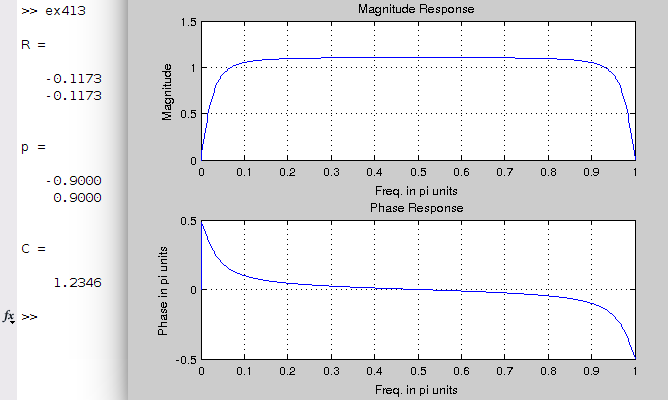
\includegraphics[width=0.5\textwidth,height=0.3\textwidth]{./images/ex413.png}
	\caption{Example 4.13 Result}
	\label{fig:Example 4.13 Result}
\end{figure}

\chapter{연습문제 4.7: }
\section{4.7-1: }
\begin {equation}
X(z) = 3z^2+2z+1-2z^{-1}+3z^{-2}, 0 < |z| < \infty
\end {equation}

\begin{lstlisting}[style=termstyle]
%Problem 4.7-1
b1 = [0 2 3]; a1 = [1]; 
[delta,n] = impseq(0,0,4);
xb1 = filter(b1,a1,delta); 
xb1 = fliplr(xb1); 
n1 = -fliplr(n);
b2 = [1 -2 -3]; 
a2 = [1]; 
xb2 = filter(b2,a2,delta); 
n2 = n;
[xa1,na1] = sigadd(xb1,n1,xb2,n2); 
xa2 = [0 0 3 2 1 -2 -3 0 0];

error = max(abs(xa1-xa2))
\end{lstlisting}

\begin{figure}[h!]
	\centering
	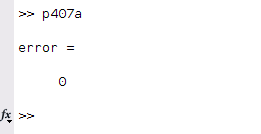
\includegraphics[width=0.3\textwidth,height=0.1\textwidth]{./images/p407a.png}
	\caption{Problem 4.7-1 Result}
	\label{fig:Problem 4.7-1 Result}
\end{figure}

\section{4.7-2: }
\begin{lstlisting}[style=termstyle]
%Problem 4.7-2

b = [0 0 0.64]; a = [1 -0.8]; 
[delta,n] = impseq(0,0,10);
xb1 = filter(b,a,delta);

[u,n] = stepseq(2,0,10); 
xb2 = ((0.8).^n).*u;

error = max(abs(xb1-xb2))
\end{lstlisting}

\begin{figure}[h!]
	\centering
	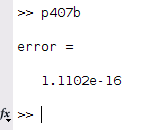
\includegraphics[width=0.3\textwidth,height=0.1\textwidth]{./images/p407b.png}
	\caption{Problem 4.7-2 Result}
	\label{fig:Problem 4.7-2 Result}
\end{figure}

\section{4.7-3: }
\begin{lstlisting}[style=termstyle]
%Problem 4.7-3

b = [ 2 0.3]; a = [1 0.3 -0.4]; 
[delta,n] = impseq(0,0,7);
xb1 = filter(b,a,delta);
[u,n] = stepseq(0,0,7); 
xb2 = (((0.5).^n).*u)+(((-0.8).^n).*u);

error = max(abs(xb1-xb2))
\end{lstlisting}

\begin{figure}[h!]
	\centering
	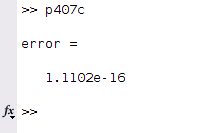
\includegraphics[width=0.3\textwidth,height=0.1\textwidth]{./images/p407c.png}
	\caption{Problem 4.7-3 Result}
	\label{fig:Problem 4.7-3 Result}
\end{figure}


\section{4.7-4: }
\begin {equation}
X(z) = \frac{1-[0.5cos(0.4\pi)]z}{1-[cos(0.4\pi)]z+0.25z^2}, |z| < 2
\end {equation}


\begin{lstlisting}[style=termstyle]
%Problme 4.7-4

b = 0.5*[2 -cos(0.4*pi)]; a = [1 -cos(0.4*pi) 0.25];
[delta,n1] = impseq(0,0,7); 
xb1 = filter(b,a,delta); 
xb1 = fliplr(xb1);

[u,n2] = stepseq(-7,-7,0); 
xb2 = ((2.^n2).*cos(0.4*pi*n2)).*u;
error = max(abs(xb1-xb2))
\end{lstlisting}

\begin{figure}[h!]
	\centering
	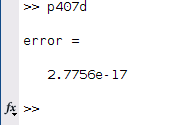
\includegraphics[width=0.3\textwidth,height=0.1\textwidth]{./images/p407d.png}
	\caption{Problem 4.7-4 Result}
	\label{fig:Problem 4.7-4 Result}
\end{figure}

\section{4.7-5: }
\begin{lstlisting}[style=termstyle]
%Problem 4.7-5

b = [1 -3]; a = [1 -9 27 -27]; 
[delta,n1] = impseq(0,0,7);
xb1 = filter(b,a,delta);
[u,n2] = stepseq(0,0,7); 
xb2 = ((n2+1).*(3.^n2)).*u;

error = max(abs(xb1-xb2))
\end{lstlisting}

\begin{figure}[h!]
	\centering
	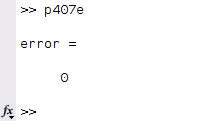
\includegraphics[width=0.3\textwidth,height=0.1\textwidth]{./images/p407e.png}
	\caption{Problem 4.7-5 Result}
	\label{fig:Problem 4.7-5 Result}
\end{figure}

\chapter{연습문제 4.12: }
deconv\_m.m:
\begin{lstlisting}[style=termstyle]
function [p,np,r,nr] = deconv_m(b,nb,a,na)
% Modified deconvolution routine for noncausal sequences
% function [p,np,r,nr] = deconv_m(b,nb,a,na)
%
% p = polynomial part of support np1 <= n <= np2
% np = [np1, np2]
% r = remainder part of support nr1 <= n <= nr2
% nr = [nr1, nr2]
% b = numerator polynomial of support nb1 <= n <= nb2
% nb = [nb1, nb2]
% a = denominator polynomial of support na1 <= n <= na2
% na = [na1, na2]
%
[p,r] = deconv(b,a);
np1 = nb(1) - na(1); np2 = np1 + length(p)-1; np = [np1:np2];
nr1 = nb(1); nr2 = nr1 + length(r)-1; nr = [nr1:nr2];
\end{lstlisting}

\begin{lstlisting}[style=termstyle]
% Problem 4.10
nb = [-2:3]; b = [1 1 1 1 1 1]; 
na = [-1:1]; a = [1 2 1];
[p,np,r,nr] = deconv_m(b,nb,a,na)
\end{lstlisting}

\begin{figure}[h!]
	\centering
	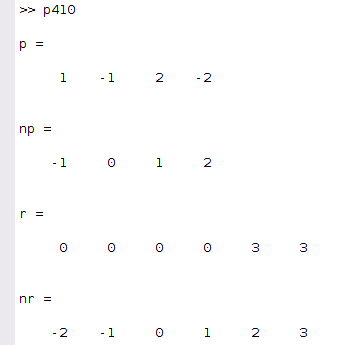
\includegraphics[width=0.5\textwidth,height=0.25\textwidth]{./images/p410.png}
	\caption{Problem 4.10 Result}
	\label{fig:Problem 4.10 Result}
\end{figure}

\chapter{연습문제 4.15: }
\section{4.15-1: }
\begin {equation}
H(z) = \frac{3}{4}+\frac{5}{4}z^{-1}+z^{-2}+z^{-3}+\frac{5}{4}z^{-4}+\frac{3}{4}z^{-5}
\end {equation}

\begin {equation}
y(n)=\frac{3}{4}x(n)+\frac{5}{4}x(n-1)+x(n-2)+x(n-3)+\frac{5}{4}x(n-4)+\frac{3}{4}x(n-5)
\end {equation}

\section{4.15-3: }


\begin{lstlisting}[style=termstyle]
%Problem 4.15

b = [3/4 5/4 1 1 5/4 3/4]; 
a = [1 0];
n = 0:200; 
x = sin(pi*n/2)+5*cos(pi*n); 
y = filter(b,a,x);

subplot(2,1,1); Hs = stem(n,x); set(Hs,'markersize',2); axis([-2 202 -7 6]);
xlabel('n'); ylabel('x(n)');
title('x(n) = sin(\pi \times n / 2)+5 \times cos(\pi \times n)');

subplot(2,1,2); Hs = stem(n,y); set(Hs,'markersize',2); axis([-2 202 -2 4]);
xlabel('n'); ylabel('y(n)');
title('Output sequence after filtering');
\end{lstlisting}

\begin{figure}[h!]
	\centering
	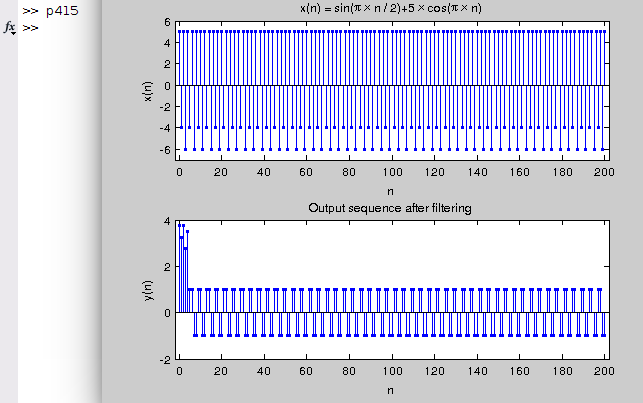
\includegraphics[width=0.7\textwidth,height=0.4\textwidth]{./images/p415.png}
	\caption{Problem 4.15 Result}
	\label{fig:Problem 4.15 Result}
\end{figure}
\end{document}

